\documentclass{beamer}
\usetheme{Copenhagen}

\expandafter\def\expandafter\insertshorttitle\expandafter{%
\insertshorttitle\hfill%
\insertframenumber}

\usepackage[frenchb]{babel} \usepackage[OT1]{fontenc}
\usepackage{lmodern} \usepackage[utf8]{inputenc}

\usepackage{amsmath,amssymb,amsthm}
\usefonttheme[onlymath]{serif}

\usepackage{hyperref}
\usepackage[squaren,Gray]{SIunits}

\usepackage{color}
\usepackage{cancel}
\usepackage{graphicx}
\usepackage{multicol}
\usepackage{enumitem}
\usepackage{tcolorbox}

\usepackage[backend=bibtex, backref=false, giveninits=true]{biblatex}
\addbibresource{biblio-stage.bib}
\renewcommand{\bibfont}{\footnotesize}

\DeclareMathOperator{\Tr}{Tr}

\begin{document}
	\author{Aurélien CARLE, Nicolas CHANON}
	\institute{Institut de Physique Nucléaire de Lyon } 
	\date{Thanks to Georgios KRINTIRAS and Chris PALMER}
	\title{Background estimation for pixel cluster counting in Van der Meer scan}
	\maketitle
	\newpage

	\begin{frame}
		\begin{block}{Noise estimation with long separation scan}
			\tiny{• Super-sep. scan 1, Jul 1 2:35-2:40 UTC. Timestamps: [1530412500, 1530412800]}
			\begin{figure}[H!]
				\begin{center}
					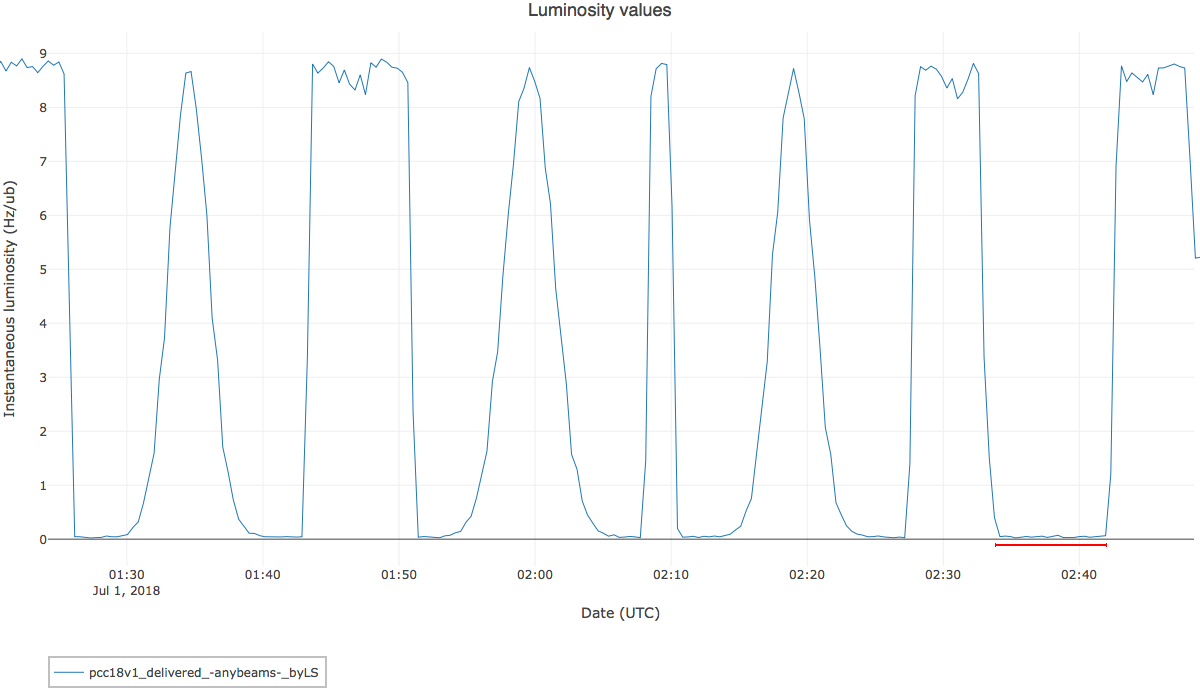
\includegraphics[scale=0.5]{longsepscan_1.png}
				\end{center}
			\end{figure}
			 \tiny{• Super-sep. scan 2, Jul 1 6:38-6:44 UTC. Timestamps: [1530427080, 1530427440]}
		
			\begin{figure}[H!]
				\begin{center}
					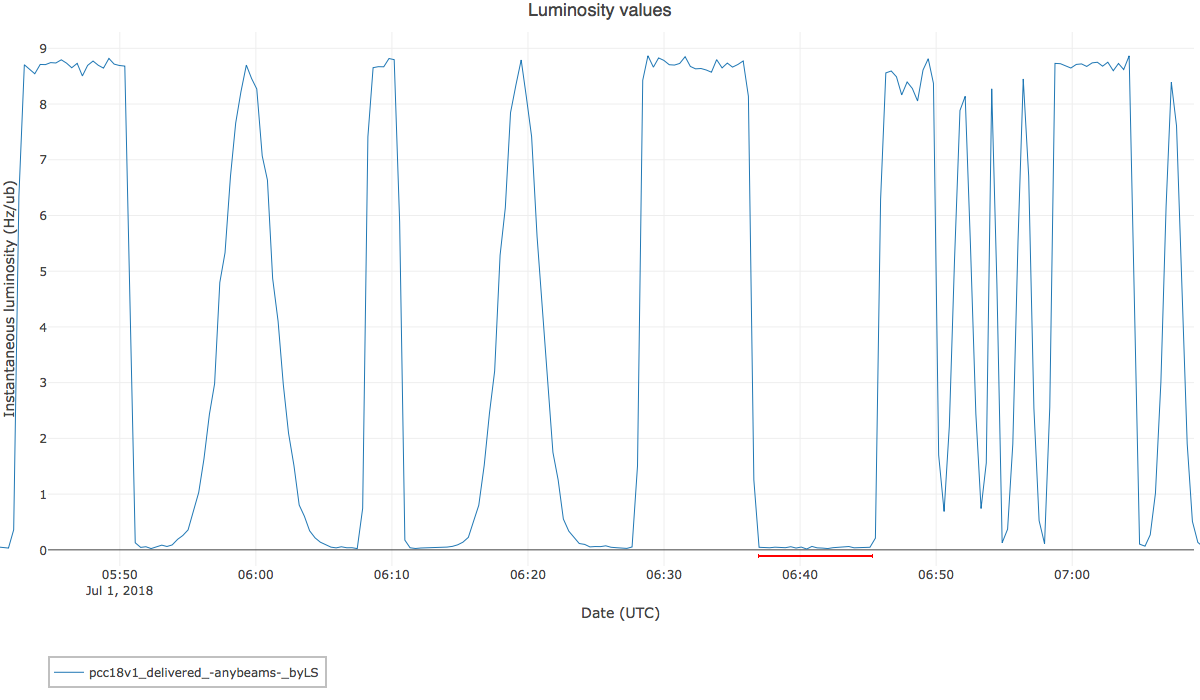
\includegraphics[scale=0.5]{longsepscan_2.png}
				\end{center}
			\end{figure}
		\end{block}
	\end{frame}

	\begin{frame}
		\begin{block}{PCC triggers in five bunch crossing (BX)}
			\begin{itemize}[label=$\triangleright$]
				\item 265, 865, 1780, 2192, 3380
			\end{itemize}
			\begin{figure}[H!]
				\begin{center}
					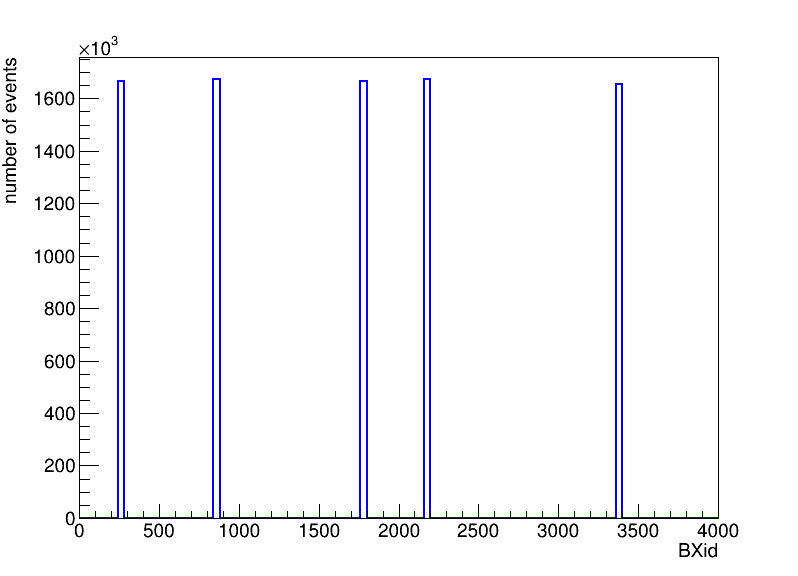
\includegraphics[scale=0.22]{BXid(1530412500<timeStamp<1530412800).png}
				\end{center}
			\end{figure}
			\begin{itemize}[label=$\triangleright$]
				\item Remove bad module list
			\end{itemize}
		\end{block}
	\end{frame}

	\begin{frame}
		\begin{block}{$\langle$nCluster$\rangle$ for time stamp range 1}
			\begin{figure}[H!]
				\begin{center}
					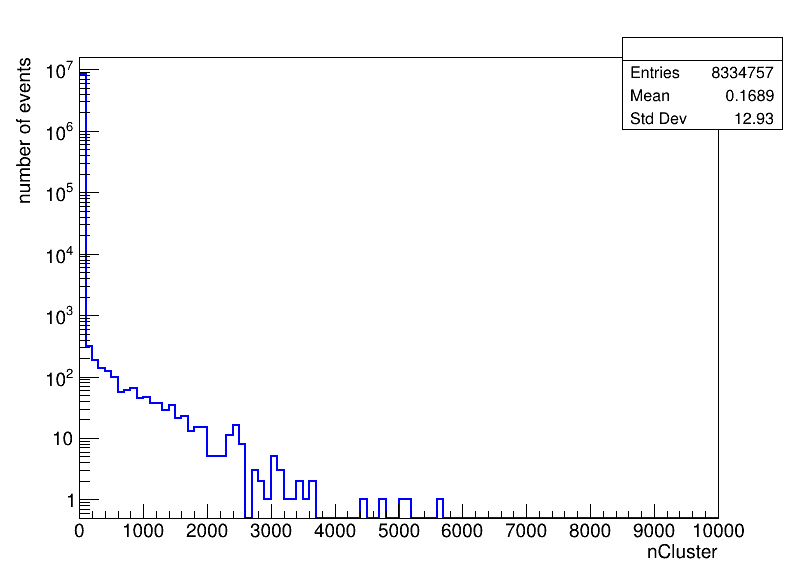
\includegraphics[scale=0.25]{nCluster(1530412500<timeStamp<1530412800).png}
				\end{center}
			\end{figure}
		\begin{center}
				$\langle$nCluster$\rangle$ = $0.169 \pm 0.005 \quad$ stat. uncertainties only
		\end{center}
		\end{block}
	\end{frame}

	\begin{frame}
		\begin{block}{$\langle$nCluster$\rangle$ for time stamp range 2}
			\begin{figure}[H!]
				\begin{center}
					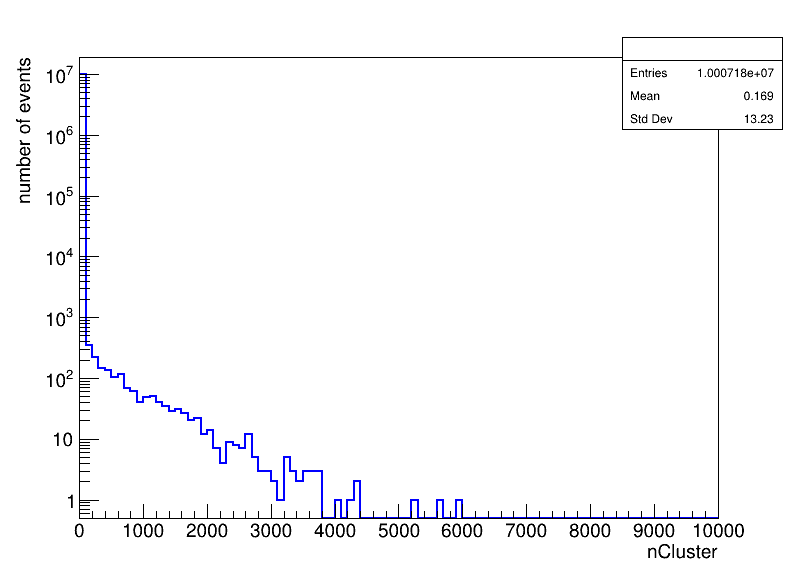
\includegraphics[scale=0.25]{nCluster(1530427080<timeStamp<1530427440).png}
				\end{center}
			\end{figure}
		\begin{center}
				$\langle$nCluster$\rangle$ = $0.169 \pm 0.004 \quad$ stat. uncertainties only
		\end{center}
		\end{block}
	\end{frame}
	
	\begin{frame}
		\begin{block}{$\langle$nCluster$\rangle$ per BX}
			\begin{center}
				Time stamp range 1 : 1530412500 $<$ timeStamp $<$ 1530412800
				\newline
				\newline
				\begin{tabular}{|c|c|}
					\hline
					BXid  & $\langle$nCluster$\rangle$ \\
					\hline
					265 & $0.18 \pm 0.01$ \\
					865 & $0.153 \pm 0.009$ \\
					1780 & $0.19 \pm 0.01$ \\
					2192 & $0.16 \pm 0.01$\\
					3380 & $0.17 \pm 0.01$\\
					\hline
				\end{tabular}
			\end{center}
		For all in time stamp range 1 :\begin{center}
		$\langle$nCluster$\rangle$ = $0.169 \pm 0.005$
		\end{center}
		\end{block}
	\end{frame}
	
	\begin{frame}
		\begin{block}{$\langle$nCluster$\rangle$ per BX}
			\begin{center}
				Time stamp range 2 : 1530427080 $<$ timeStamp $<$ 1530427440
				\newline
				\newline
				\begin{tabular}{|c|c|}
					\hline
					BXid  & $\langle$nCluster$\rangle$  \\
					\hline
					265 & $0.170 \pm 0.009$ \\
					865 & $0.176 \pm 0.009$\\
					1780 & $0.19 \pm 0.01$\\
					2192 & $0.134 \pm 0.007$\\
					3380 & $0.18 \pm 0.01$\\
					\hline
				\end{tabular}
			\end{center}
				For all in time stamp range 2 :\begin{center}
			$\langle$nCluster$\rangle$ = $0.169 \pm 0.004$
		\end{center}
		\end{block}
		\begin{block}{For all in the two time stamp ranges}
			\begin{center}
			$\langle$nCluster$\rangle$ =	$0.169 \pm 0.003$
			\end{center}
		\end{block}
	\end{frame}	

	\begin{frame}
		\begin{block}{Variation within the scan (to illustrate)}
			All the time stamp ranges in same plot : 
			\begin{figure}[H!]
				\begin{center}
					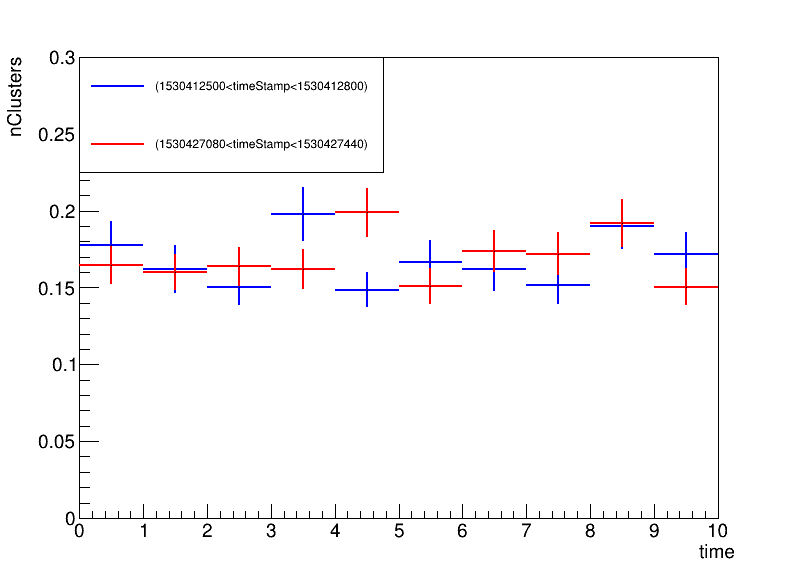
\includegraphics[scale=1]{nClusterBin.png}
				\end{center}
				\tiny{(In this plot, bins do not represent the same duration for timestamp ranges 1 and 2)}
			\end{figure}
		\end{block}
	\end{frame}


	\begin{frame}
		\begin{block}{Variation within the scan}
			Time stamp range 1 :
			\begin{figure}[H!]
				\begin{center}
					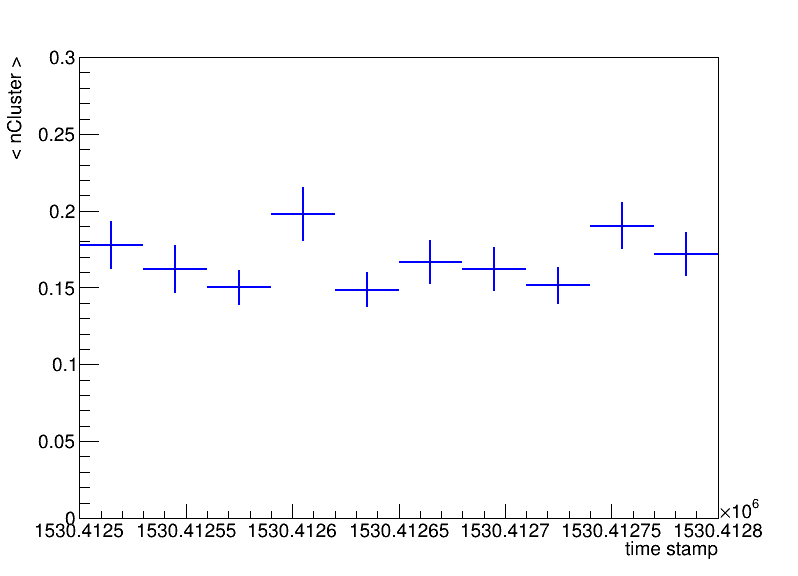
\includegraphics[scale=0.25]{timeStampAverageCluster(1530412500<timeStamp<1530412800).png}
				\end{center}
			\end{figure}
		\end{block}
	\end{frame}

	\begin{frame}
		\begin{block}{Variation within the scan}
			Time stamp range 2 :
			\begin{figure}[H!]
				\begin{center}
					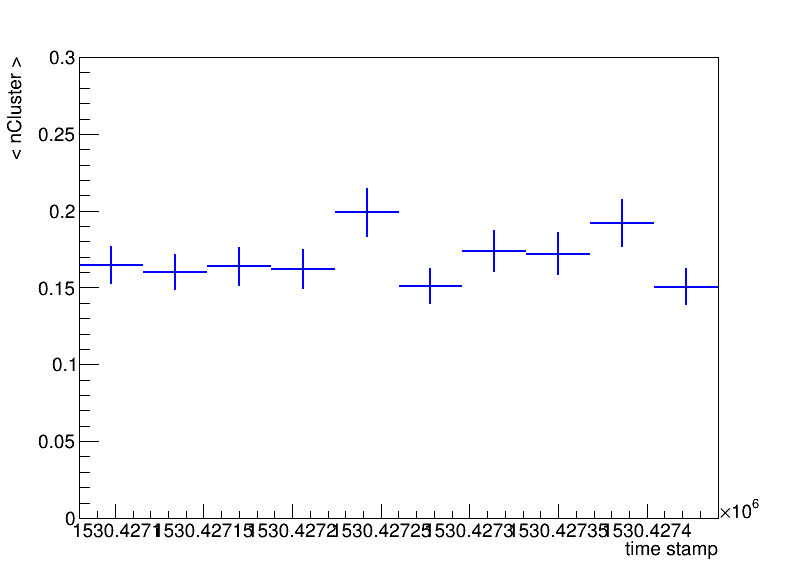
\includegraphics[scale=0.25]{timeStampAverageCluster(1530427080<timeStamp<1530427440).png}
				\end{center}
			\end{figure}
		\end{block}
	\end{frame}
	
	\begin{frame}
		\begin{block}{Ratio Background / Head-On value}
			\begin{itemize}[label=$\triangleright$]
				\item Compare background value with head-on value of $\langle$nCluster$\rangle$
			\end{itemize}
			\begin{columns}
				\begin{column}{4.2cm}
					\begin{figure}[H!]
						\begin{center}
							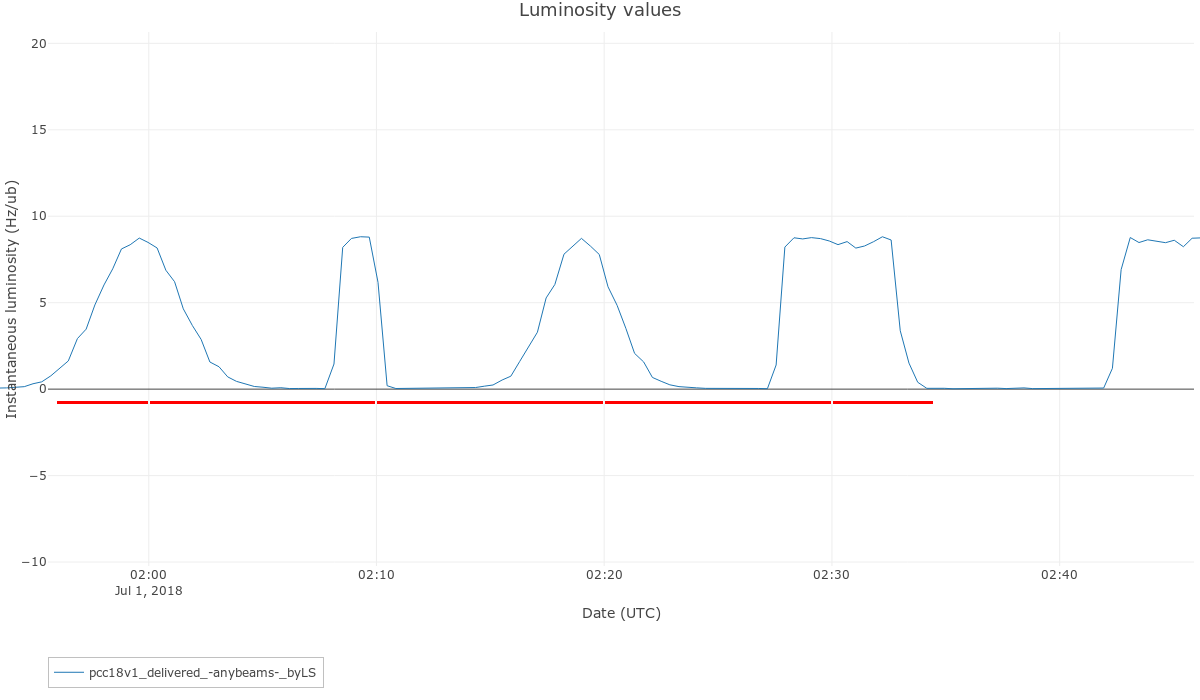
\includegraphics[scale=0.5]{longsepscan_3.png}
						\end{center}
					\end{figure}	
				\end{column}
				\begin{column}{5.5cm}
					\begin{figure}[H!]
						\begin{center}
							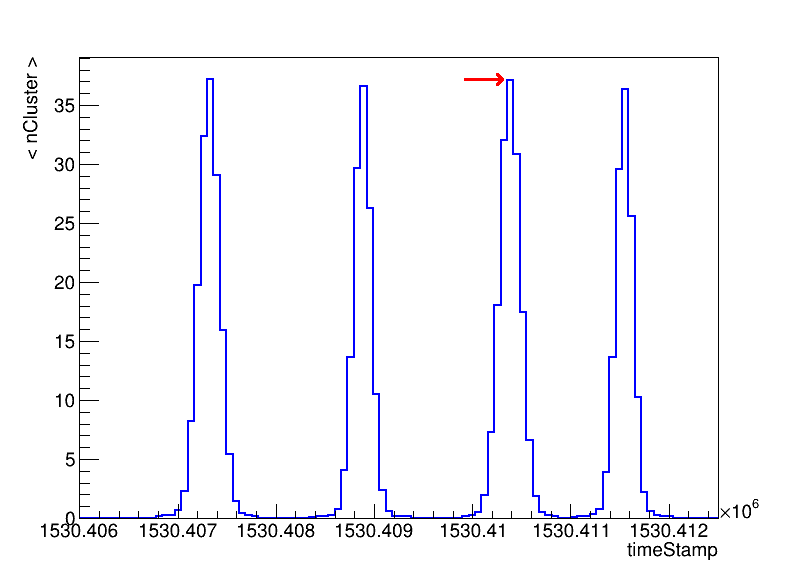
\includegraphics[scale=0.83]{Signal.png}
						\end{center}
					\end{figure}	
				\end{column}
			\end{columns}
			\begin{itemize}[label=$\triangleright$]
				\item Ratio is : $0.45 \%$
			\end{itemize}
		\end{block}
	\end{frame}


\end{document}	